% This is samplepaper.tex, a sample chapter demonstrating the
% LLNCS macro package for Springer Computer Science proceedings;
% Version 2.20 of 2017/10/04
%
\documentclass[runningheads]{llncs}
%
\usepackage{graphicx}
\usepackage{amsmath}
\usepackage{amssymb}
% Used for displaying a sample figure. If possible, figure files should
% be included in EPS format.
%
% If you use the hyperref package, please uncomment the following line
% to display URLs in blue roman font according to Springer's eBook style:
% \renewcommand\UrlFont{\color{blue}\rmfamily}

\begin{document}
%
\title{CS3243 Project 1 - $k$-puzzle}
%
\titlerunning{CS3243 Project 1}
% If the paper title is too long for the running head, you can set
% an abbreviated paper title here
%
\author{Chen Yuanbo \and
Ho Wei Haw \and
Lee Liak Ghee \and
Liu Zechu}
%
\authorrunning{F. Author et al.}
% First names are abbreviated in the running head.
% If there are more than two authors, 'et al.' is used.
%
\institute{National University of Singapore \\
\url{https://github.com/ybchen97/3243project1}}
%
\maketitle              % typeset the header of the contribution
%
\begin{abstract}
This paper outlines our findings and comparisons of various uninformed and informed search algorithms for solving the k-puzzle. In particular, we will be comparing various heuristics for A* search against each other and the uninformed search algorithm. 

\keywords{uninformed search \and informed search}
\end{abstract}
%
%
%
\section{Problem Specification}
Let $k \in \mathbb{N}$, $k \geq 2$ and denote $ S = \{ i : 0 \leq i \leq k^2 - 1 \}$. We will use the number $0$ to represent the blank tile.

\subsection{State Representation}
A state is represented as a $1 \times k^{2}$ row vector $v$ with distinct elements from $S$. More precisely, if the original puzzle is seen as a $k \times k$ matrix $A = \left( a_{ij} \right)$ with $1 \leq i,j \leq k$, then under our representation, its corresponding row vector is given by the entries $ v_{k(i - 1) + j} = a_{ij} $. The goal state is thus given by $v_g = \left( 1, \ 2,\ ..., \ k^2 - 1, \ 0 \right)$.

\subsection{Actions}
To define the actions, we will denote the index of the blank tile in our state representation as $i_0$. This gives us the following formulations:

\begin{enumerate}
    \item A legal ``UP'' action occurs when $i_0 < k^{2} - k$ and swaps the tile at the index $i_0 + k$ with the blank tile.
    
    \item A legal ``DOWN'' action occurs when $i_0 > k - 1$ and swaps the tile at the index $i_0 - k$ with the blank tile.
    
    \item A legal ``LEFT'' action occurs when $i_0 \not\equiv k - 1 \pmod{k}$ and swaps the tile at the index $i_0 + 1$ with the blank tile.
    
    \item A legal ``RIGHT'' action occurs when $i_0 \not\equiv 0 \pmod{k}$ and swaps the tile at the index $i_0 - 1$ with the blank tile.
\end{enumerate}

\subsection{Transition Model}
If $r$ is the current state and $r'$ is the new state after a legal action $a$ is performed, our transition model $T$ is given by $ T(r, a) = r' $
where the entries of $r'$ are exactly the same as $r$ except for the 2 tiles that are being swapped. 

\section{Technical Analysis of Search Algorithms and Heuristics}
In our analysis, we will be adopting these notations: 
\begin{enumerate}
    \item $b$, the maximum branching factor. In this problem, $b = 4$ since there are at most $4$ possible actions at each state.
    \item $s$ and $s'$, the current state and a successor of $s$ respectively.
    \item $d$, the depth of the shallowest solution
    \item $c(s, s')$, the cost of going from $s$ to $s'$. This is always equal to 1 in the $k$-puzzle since only 1 move can be made at each time.
\end{enumerate}

Next,we note that for a given $k$-puzzle, there are at most $k!$ states in the search space. As this is a finite search space, all of our algorithms are guaranteed to be $\mathbf{complete}$. Besides that, to detect for unsolvable initial states quickly, we made use of ideas from \cite{ref_1}. 

\subsection{Breadth First Search (BFS)}
BFS is guaranteed to provide an optimal solution since all step costs are identical. Furthermore, both the time and space complexity are given by $O(4^d)$.

\subsection{A* Search - Euclidean Distance}
This heuristic (denoted as $h_1$) calculates the sum of the straight line distance each non-blank tile is away from the goal position. This gives us our first proposition.

\begin{theorem} 
$h_1$ is consistent.
\end{theorem}

\begin{proof}
Firstly, moving a single tile $t$ does not change the Euclidean distance of the remaining tiles from their goal state. So, it suffices to only consider the distance of the tile being moved. Furthermore, this move will change either only the horizontal distance or the vertical distance of $t$ by $\pm 1$. WLOG, we can assume that there is a horizontal change. 

If there is a positive horizontal change, by denoting the current coordinate of $t$ as $(x_t, y_t)$ in the grid, we note that $x_{t}^{2} + y_{t}^{2} \leq \left( x_{t} + 1 \right)^{2} + y_{t}^2$. This implies that $h_1(s) \leq h_1(s')$ and so, $h_1(s) \leq c(s, s') + h_1(s')$.

Now, if there is a negative horizontal change, we wish to show that the following inequality holds:
\begin{equation}
    \sqrt{x_{t}^{2} + y_{t}^{2}} \leq \sqrt{(x_{t} - 1)^{2} + y_{t}^{2}} + c(s, s') = \sqrt{(x_{t} - 1)^{2} + y_{t}^{2}} + 1
\end{equation}
Since all the terms involved are positive, performing algebraic manipulation on $(1)$ yields an equivalent inequality $0 \leq y^{2}$ which is obviously true. Thus, $(1)$ has to be true and it follows that $h_{1}(s) \leq c(s, s') + h_1(s')$. The proof for a vertical change is similar and this proves our claim.
\end{proof}

\subsection{A* Search - $\max($Relaxed Adjacency, Manhattan Distance$)$}
This heuristic involves taking the maximum of 2 heuristics, the Relaxed Adjacency heuristic (which counts the minimum number of swaps with the blank tile needed to reach the goal state) and the Manhattan Distance heuristic and is adapted from \cite{ref_2}. 

However, a proof of consistency of the Relaxed Adjacency heuristic is not provided in \cite{ref_2}. As such, we will provide a proof sketch as the proof we came up with is rather lengthy. Each state can be seen as a permutation of numbers and thus, can be expressed as a product of disjoint cycles. Moving a tile to the blank tile will either join $2$ of these cycles or break up a single cycle. This causes the minimum number of swaps to change by a value of $\pm 1$. Since $c(s, s') = 1$, this eventually causes $h(s) \leq c(s, s') + h(s')$. The full proof can be found in the Appendix.

Next, the reason for taking the maximum value of both heuristic is that there are instances where one of the heuristic is larger than the other. For instance, for $k = 3$, we have the following examples:
\begin{center}
    \begin{tabular}{| c | c | c |}
        \hline
        1 & 3 & 2 \\
        \hline
        4 & 5 & 6 \\
        \hline
        7 & 8 & 0 \\
        \hline
    \end{tabular}
    \quad
    \begin{tabular}{| c | c | c |}
        \hline
        8 & 2 & 3 \\
        \hline
        4 & 6 & 5 \\
        \hline
        7 & 0 & 1 \\
        \hline
    \end{tabular}
\end{center}

In the left grid, Manhattan Distance gives a value of $2$ while Relaxed Adjacency gives a value of $3$. In the right grid, Manhattan Distance gives $9$ while Relaxed Adjacency gives $5$.

Lastly, since both of the heuristics are consistent, the maximum of them is consistent. Indeed, if $h$ and $h'$ are consistent heuristics, then
\begin{align*}
    h(s) & \leq c(s, s') + h(s') \leq c(s, s') + \max (h(s'), h'(s'))\\
    h'(s) & \leq c(s, s') + h'(s') \leq c(s, s') + \max (h(s'), h'(s')) 
\end{align*}
and so the maximum of them is consistent too.

\subsection{A* Search - Linear Conflict}
Our last heuristic is also adapted from the paper in \cite{ref_2}. In essence, this heuristic calculates the additional steps that have to be taken in order to resolve conflicts in both the rows and columns in addition to the Manhattan distances. Two tiles are said to be in conflict if they and their goal positions are currently in the same line but both are blocking the other from reaching their goals. A detailed discussion and full proof of its consistency is also provided in \cite{ref_2}.

\section{Experimental Set Up for Performance Evaluation}
\subsection{Evaluation Criteria}
\subsection{Measurement of Performance Metrics}
\section{Results and Discussion}


\begin{table}
\caption{Table captions should be placed above the
tables.}\label{tab1}
\begin{tabular}{|l|l|l|}
\hline
Heading level &  Example & Font size and style\\
\hline
Title (centered) &  {\Large\bfseries Lecture Notes} & 14 point, bold\\
1st-level heading &  {\large\bfseries 1 Introduction} & 12 point, bold\\
2nd-level heading & {\bfseries 2.1 Printing Area} & 10 point, bold\\
3rd-level heading & {\bfseries Run-in Heading in Bold.} Text follows & 10 point, bold\\
4th-level heading & {\itshape Lowest Level Heading.} Text follows & 10 point, italic\\
\hline
\end{tabular}
\end{table}


\noindent Displayed equations are centered and set on a separate
line.
\begin{equation}
x + y = z
\end{equation}
Please try to avoid rasterized images for line-art diagrams and
schemas. Whenever possible, use vector graphics instead (see
Fig.~\ref{fig1}).

\begin{figure}
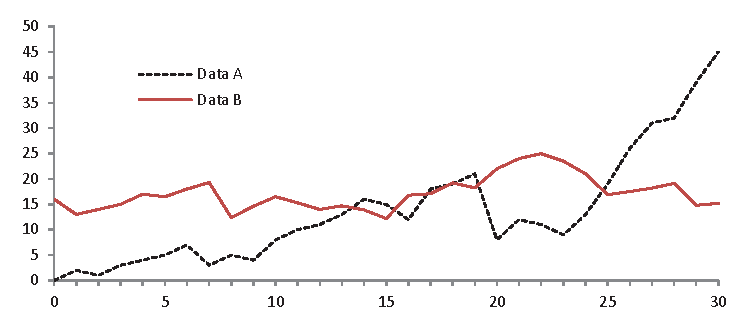
\includegraphics[width=\textwidth]{fig1.eps}
\caption{A figure caption is always placed below the illustration.
Please note that short captions are centered, while long ones are
justified by the macro package automatically.} \label{fig1}
\end{figure}

%
% ---- Bibliography ----
%
% BibTeX users should specify bibliography style 'splncs04'.
% References will then be sorted and formatted in the correct style.
%
% \bibliographystyle{splncs04}
% \bibliography{mybibliography}
%
\begin{thebibliography}{8}
\bibitem{ref_1}
Solvability of the Tiles Game,
\url{https://www.cs.bham.ac.uk/~mdr/teaching/modules04/
java2/TilesSolvability.html}.
Last accessed 23 Feb 2020

\bibitem{ref_2}
Hansson, O., Mayer, A. E., Yung, M. M.. Generating Admissible Heuristics by Criticizing Solutions to Relaxed Models (1985)
\end{thebibliography}

\section{Appendix}
In Section 2.3, we claimed that the Relaxed Adjacency heuristic is consistent. We will now provide a full proof for our claim. However, we will make use of the following ideas from Group Theory.

A permutation on a set $S$ is a bijection from $S$ to itself. In particular, we will be considering permutations on a set $S = \{1, 2, ..., k^2 - 1, 0\}$ where $n$ is a positive integer. One interesting fact about this kind of permutations is that if we are to take its corresponding function $f$ and apply it repeatedly on one number $x \in S$, we obtain a sequence as such:
$$
x \to f(x) \to f^{2}(x) \to ... \to f^{m}(x)
$$
Since $S$ is finite, this sequence has to go back to $x$ at some point of time. All of the distinct numbers in the above sequence are called a $\mathbf{cycle}$. As an illustration, we consider the permutation $f$ given by
\begin{equation*}
    \begin{pmatrix}
    1 & 2 & 3 & 0 \\
    2 & 1 & 3 & 0
    \end{pmatrix}
\end{equation*}
where $f$ takes the elements in the first row and mapped it to the corresponding element in the second row. It can be easily verified that $\{ 1, 2\}$ forms a cycle while the singleton sets $\{3\}$ and $\{0\}$ are also a cycle. This gives rise to the $\mathbf{cycle \ notation}$ of the permutation $f$: $(1 \ 2)$ where $(1 \ 2)$ means that $f(1) = 2$ and $f(2) = 1$. Elements that are not moved are omitted from the cycle representation of the permutation. Furthermore, we note that each of these cycles are $\mathbf{disjoint}$. With these ideas, we can now state certain theorems from Group Theory which will help us in our proof of consistency:

\

$\mathbf{Fact \ 1}$: Any permutation can be represented as a product of disjoint cycles.

\

$\mathbf{Fact \ 2}$: Consider the permutations, with $i < j$, in their disjoint cycles representation.
\begin{align*}
\sigma &= (x_1 \ x_2 \ ... \ x_{i - 1} \ x_{i} \ ... \ x_{j - 1} \ x_{j} \ ... x_{k}) \\
\tau &= (x_1 \ x_2 \ ... \ x_{i - 1} \ x_{j} \ ... \ x_{k})(x_{i} \ x_{i + 1} \ ... \ x_{j - 1})
\end{align*}
Then $(x_{i} \ x_{j})\sigma = \tau$ and $(x_{i} \ x_{j})\tau = \sigma$. In other words, swapping $2$ elements in a single cycle breaks up the cycle into $2$ disjoint cycles.In particular, using the above notation, they are broken into cycles of length $j - i$ and $k - j + i$ where length denotes the number of elements in the cycle. Likewise, swapping $2$ elements in $2$ disjoint cycles connect them together as a single cycle.

\

 As mentioned in Section 2.3, the state of the puzzle as a permutation of the numbers $1, 2, ..., k^{2} - 1, 0$. As an example, for $k = 3$, the following state
\begin{center}
    \begin{tabular}{|c|c|c|}
    \hline
    3 & 4 & 2 \\
    \hline
    1 & 0 & 8 \\
    \hline
    7 & 5 & 6 \\
    \hline
    \end{tabular}
\end{center}
can be seen as the permutation $(3, 4, 2, 1, 0, 8, 7, 5, 6)$ whose cycle representation is given by $(1 \ 3 \ 2 \ 4)(5 \ 0 \ 6 \ 8)$. The goal state is given by the permutation $(1, 2, 3, 4, 5, 6, 7, 8, 0)$. We now establish another $2$ facts which are reproduced from $\cite{ref_2}$ for easier reference.

\

$\mathbf{Fact \ 3}$: If a cycle of the form $(t_{1} \ ... \ t_{m})$ in the state contains the number $0$, then it requires a minimum of $m - 1$ swaps with the blank tile to return the numbers to the original position.
    
\

$\mathbf{Fact \ 4}$: If a cycle of the form $(t_{1} \ ... \ t_{m})$ in the state does not contain the number $0$, then it requires a minimum of $m + 1$ swaps with the blank tile to return the numbers to the original position.

\

We are now ready to prove the consistency of the Relaxed Adjacency heuristic.

\begin{theorem}
The Relaxed Adjacency heuristic, denoted as $h_3$, is consistent.
\end{theorem}

\begin{proof}
Let $s$ be the current state of the puzzle, $s'$ be any of its successor and $c(s, s')$ be the cost of moving from $s$ to $s'$. Using our permutation representation above, by Fact 1, we can break it into a product of disjoint cycles $\tau_1 \tau_2 ... \tau_m$. We now consider $2$ cases.

\

$\mathbf{Case \ 1}$: $k^2$ is not part of any of the disjoint cycles, that is, $k^2$ is in its correct position. By Fact $4$, we have 

$$
h_3(s) = \sum_{1 \leq i \leq m} (l_{i} + 1)
$$
where $l_i$ denotes the length of $\tau_{i}$. Now, moving a tile to the blank tile gives rise to $2$ possibilities:

\

$\mathbf{Case \ 1.1}$: A tile $t$ not in any of the $\tau_i$ is moved to the blank tile. In other words, $t$ is in its correct position. By Fact 2, this move creates a cycle $(t \ k^{2})$ of length $2$. It follows from Fact 3 that this cycle requires $1$ swap to swap it back. Thus, we have

$$
h_3(s') + c(s, s') = \sum_{1 \leq i \leq m} (l_i + 1) + 1 + 1 \geq h_3(s)
$$

$\mathbf{Case \ 1.2}$: A tile $t$ from one of the $\tau_i$ is moved to the blank tile, call it $\tau_j$. By Fact 2, this creates a cycle of length $l_j + 1$ which by Fact 3, requires $l_j$ swaps to return it to its original position. Thus,

$$
h_3(s') + c(s, s') = \sum_{\substack{1 \leq i \leq m \\ i \neq j}} (l_i + 1) + l_j + 1 = \sum_{1 \leq i \leq m} (l_i + 1) = h_3(s)
$$

$\mathbf{Case \ 2}$: $k^2$ is in one of the disjoint cycles, call it, $\tau_j$. By Fact 4, we have

$$
h_3(s) = \sum_{\substack{1 \leq i \leq m \\ i \neq j}}(l_i + 1) + l_j - 1
$$
Once again, we have the following possibilities after moving a single tile.

\ 

$\mathbf{Case \ 2.1}$: The tile being moved to the blank tile is part of $\tau_j$. Once again, we have the following 2 subcases to consider.

\ 

Subcase (a): The move taken is part of the $l_j - 1$ moves required to return the elements in the cycle to their original positions. Then, we note that

$$
h_3(s') + c(s, s') = \sum_{\substack{1 \leq i \leq m \\ i \neq j}} (l_i + 1) + (l_j - 2) + 1 = h_3(s).
$$

\

Subcase (b): The move taken is not part of the $l_j - 1$ moves required to return the elements in the cycle to their original positions. Then, this breaks the cycle into 2 disjoint cycles by Fact 2, with length $a$ and $l_j - a$ respectively, $0 < a < l_j$. Since one of these cycles contain the blank tile and the other contains no blank tile, by Facts 3 and 4, the total number of swaps needed to return these 2 disjoint cycles back is $l_j$. This gives

$$
h_3(s') + c(s, s') = \sum_{\substack{1 \leq i \leq m \\ i \neq j}} (l_i + 1) + l_j + 1 > h_3(s)
$$

\ 

$\mathbf{Case \ 2.2}$: The tile being moved to the blank tile is not part of $\tau_j$. Suppose that tile is instead part of the cycle $\tau_{j'}$. By Fact 2, this creates a new cycle of length $l_j + l_{j'}$ with the blank tile being part of it. By Fact 3, this requires $l_j + l_{j'} - 1$ moves to return to its goal positions. Thus,

$$
h_3(s') + c(s, s') = \sum_{\substack{1 \leq i \leq m \\ i \neq j \\ i \neq j'}}(l_i + 1) + (l_j + l_{j'} - 1) + 1 
= \sum_{\substack{1 \leq i \leq m \\ i \neq j}}(l_i + 1) + l_j - 1 
= h_3(s)
$$

\

We note that in all possible cases, we have 
$$
h_3(s) \leq h_3(s') + c(s, s') 
$$
and this concludes the proof.

\end{proof}
\end{document}
